
% !TEX TS-program = pdflatex
% !TEX encoding = UTF-8 Unicode

%************************************************
\chapter{La composizione: Insinuarsi nel vuoto}
\label{chp:La composizione: Insinuarsi nel vuoto}
%************************************************

\epigraph{[...] è sempre quel vuoto dell’intervallo complesso, che fa il volume ulteriore, un vuoto che collega non un vuoto che separa. \\
Giorgio Netti, Masterclass EmuFest IX, 2016 \textit{Conservatorio Santa Cecilia}, Roma}


\textit{Insinuarsi nel vuoto} è una composizione che si divide in due parti, nominate varchi, e rappresenta in qualche modo il mio percorso compositivo degli ultimi anni. Il primo, \textit{L'albe nei varchi} appunto, è un brano per sassofono soprano, tape ed elaborazione tramite riverberi; il secondo è \textit{Insinuarsi, mosso contrario}, un solo per Unamolla e \textit{live electronics} che sfocia in un duo con il sassofono tenore: Unamolla, sassofoni e live electronics racchiudono un processo di studi fatto su strumenti musicali di liuteria classica e strumenti di nuova creazione.
\\ \\
I varchi, non vanno immaginati di fronte, come se si dovesse attraversarli, ma ai lati. Come nel caso di Bologna o di Torino, dove le arcate sono laterali. Ogni passo è un ascolto, ogni passo verso il centro è sempre piú incalzante, finché, non ci si rende conto che la via è lunga e il tutto si bagna di una luce nuova. 
La luca nuova, E2. rappresenta una planimetria intrinseca dello strumento. Si va ad indagare nel lontano passato di suono, per il momento sconosciuti. Non ci sono più artefatti, è il suono che prende forma, è il tempo che si dilata: il vuoto non è più intrinseco ma diventa formale, il vuoto è lo spazio nel quale il suono si disperde e questo vuoto, risuona. Diventa risuonatore incostante di un precipitare che si tramuta in tempo-frequenza tempo-timbro e tempo-dinamica. L’incostante sempre uguale senso della vita che crea la normalità. Dove da una parte c’è chi riesce a viversi questa discesa senza pensare e chi è in ascolto, sente la continua vibrazione dell’aria che colpisce il corpo nella caduta. Insinuarsi nel vuoto è questa caduta che non trova mai il suolo, ma nell’aprire gli occhi trova il buio e una continua brezza sulla pelle che fa il vivere e non il sopravvivere.
E mi dirigo verso il nuovo, verso lo sconosciuto e nel vuoto dello spazio che sta tra le spire si incastrano i crini dell’arco nella ricerca di una vocalità che resa all’interno della molla ed enfatizzata echeggia, si disperde. Come si disperde l’aria all’interno del sassofono, come il fiato si trasforma in suono che dalla cavità orale viene filtrato dall’ancia e della labbra per penetrare nel tubo, apparentemente vuoto. 

%************************************************

\section{Varco I: L'albe \textit{come fuggir nel susseguir d'incanti}}

È il primo quadro ideato per raccontare, tramite le composizioni e non nelle composizioni, un percorso musicale o, se si vuole, di vita, dove, attraverso l’utilizzo di tecniche compositive e quindi gestuali, si indica un cammino compositivo formale. La parte scritta per sassofono soprano è legata ad uno studio fatto sul Trattato II - Netti Weiss, dove utilizzo varie figure presenti nel libro che si legano ad una parte di elettronica ideata sull’elaborazione di parti vocali sul \textit{Sol} e \textit{Sib} dell'ottava del Do centrale.
I varchi, non vanno immaginati come attraversati, ma nelle parti laterali di un viale coperto. Come nel caso di Bologna o di Torino, cove le arcate sono laterali a questi tunnel. Ogni passo è un ascolto è una trasformazione, ogni passo verso il centro è sempre più incalzante, finché non ci si rende conto che la via è lunga e il tutto si bagna di una luce nuova. \\
La luce nuova è l'elaborazione nei riverberi, è la tecnica estesa, è il finale del brano, dove all'interno del tape entra un campione di sassofono, ricampionato ad una frequenza di campionamento più alta e questo rende possibile la dilatazione temporale del campione che tramite un fade-out muore nell'inizio della seconda parte.

\subsection{Attese, silenzio e spazi.}

Come sostiene Paolo Mauri, critico letterario e storico della letteratura, in \textit{Buio}:
\begin{quotation}
Buio e silenzio. Tra le due parole c’è un legame antico, anche se [...] non obbligatorio. Molti sono esploratori del silenzio che fatalmente incontrano anche il buio. Sul silenzio notturno riflette e scrive più volte Leopardi, che è un vigile guardiano della notte oltre che uno scrutatore appassionato del cielo stellato. Il silenzio notturno può portare orrore o quiete. Il sonno si coniuga anch’esso al buio e con il sonno il sogno, quest’altra misteriosa metà della vita umana che sfugge al nostro controllo e che forse, invece, ci controlla, liberando i nostri demoni interiori, le nostre anche e anche i nostri desideri. \\
Il buio tuttavia può essere anche riempito di rumori, di suoni, per esempio di musica. Allora noi entriamo consapevolmente nel buio alla ricerca di sensazioni e di emozioni. Le discoteche e anche i vecchi night quei luoghi, privi del suono e degli effetti speciali, perdono completamente di senso e di identità\footnote{Paolo Mauri, \textit{Buio}, Casa editrice Einaudi, Trento, aprile 2007}.
\end{quotation}
Il silenzio è stata una pratica musicale molto in auge negli anni ‘60. Fisicamente il silenzio non è possibile, perché se c’è movimento nei corpi (ad esempio respirazione) o movimento al di fuori (aria in movimento) creare il silenzio è praticamente impossibile. Si può però indurre un’ascoltatore a tale suggestione, se in precedenza troviamo un crescendo o semplicemente se prima c’è del suono e dopo viene a mancare. \\
Alcune pratiche di ascolto, come il giradischi o il lettore cassette o spesso il CD, sono legate ad un rumore di fondo fisso, dato da vari fattori fisici dello strumento stesso\footnote{il nastro ha un rumore di fondo alto, il giradischi ha comunque dei solchi e così via}, quindi, l’evoluzione nell’utilizzo all’interno della musica eseguita dal vivo in sistemi digitali, ha reso possibile passare da un sistema analogico, perciò infinito a un sistema digitale e finito. Il sistema digitale ha come lato positivo che è utilizzabile, con un’adeguata strumentazione, per indurre al “silenzio relativo”.
L’albe nei varchi è una composizione che gioca su questi interruttori, con i dovuti crescendo e diminuendo. \\
L'impossibilità di eseguibilità data dalle misure restrittive in auge in questo momento, mi hanno fatto decidere di operare diversamente. In seguito spiegherò le modalità con le quali ho concluso e realizzato il brano, fornendo alla commissione una versione \textit{studio} del mio brano. 

\subsection{Il rapporto con lo strumentista}

Il rapporto con lo strumentista è una fase fondamentale per la stesura del pezzo. Ogni strumento è differente dall'altro e anche la cassa toracica e le labbra di chi esegue il pezzo. Dico questo per osservare che a volte le posizioni presenti sui trattati\footnote{In questo caso il \textit{Netti-Weiss}} sono specifiche per l'esecutore che le ha eseguite e variano anche in modo minimo per un altro strumentista. \\
Il passaggio fatto è stato il seguente: stesura della partitura con le notazioni di Giorgio Netti ed in seguito invio del materiale al mio strumentista Danilo Perticaro. Danilo ha studiato la parte, redatto le giuste modifiche. Cambiata in seguito la partitura, ho inviato di nuovo il materiale a Danilo per l'accertamento delle correzioni.

\subsection{Il lavoro a distanza}

Importante ed essenziale è stata la presenza a distanza dello strumentista. Dopo aver chiesto al maestro Giorgio Netti di poter utilizzare le sue registrazioni\footnote{su internet sono presenti le registrazioni di ogni singolo multifonico presente nel trattato} per creare un missato tale da poter elaborare ed ideare l'elettronica, ho inviato il lavoro ultimato del tape e dell'elaborato stereo finale, per dare così a Perticaro la giusta suggestione e la precisa direzione musicale che volevo raggiungere. \\
Eseguite le parti, Danilo mi ha inviato un file nel quale era presente il suo sassofono e l'ho sostituito all'interno della mia workstation digitale. Ho proposto all'esecutore una registrazione continua e totale del pezzo, così da fargli assumere una continuità, con tutte le possibilità del caso: rumore di chiavi, respiri, intenzione. 

%************************************************

\section{Varco II: Insinuarsi nel vuoto, \textit{mosso contrario}}

\epigraph{
sólo agg. e avv. [lat. sōlus, e come avv. sōlum e poi sōlō]. – 1. agg. a. Di persona, che è senza compagnia di alcuno, che non ha nessun altro insieme o vicino: Solo e pensoso i più deserti campi Vo mesurando a passi tardi e lenti (Petrarca) [...] \\ \textit{dall'Enciclopedia online www.treccani.it}}


Se nel primo varco ho voluto fare interagire uno strumento di liuteria classica con un tape elettronico di elaborazione di un campione, nel secondo varco ho deciso di utilizzare Unamolla e solo nella parte finale avviene il connubio con il sassofono tenore. Unamolla\footnote{come abbiamo visto nel capitolo 2} è uno strumento, per il momento, inarmonico. Questo strumento viene elaborato e modificato nel suo corso di esecuzione, tramite 7 canali che \textit{splittano\footnote{ovvero, moltiplicano il canale mono in 7 canali differenti elaborati ognuno con un processo a sé stante}} il segnale, in 7 parti, per ricreare un eterno ritorno, ma nel ritorno c’è una modifica continua, proprio come indicava Nono con la sua nostalgia del futuro:

\begin{quotation}
[...]evoluzione e rivoluzione, due fasi strettamente conseguenti: mercé le cui forze propulsive, e specie quella anche violenta della seconda in cui violenza altro non è se non ampliamento della capacità umana, si attua la umana continuità. \\
la vita si realizza in forma talmente viva, ché il presente è già il passato nel futuro. \\
in modo analogo, ma da analizzare ogni volta concretamente nella diversità della sua concreta situazione, procede tra spazi tra suoni tra colori l'uomo-poeta\footnote{Luigi Nono, \textit{La nostalgia del futuro, Scritti scelti 1948-1986}, Gruppo editoriale Il Saggiatore s.p.a., Milano 2007}.
\end{quotation}

\subsection{La nostalgia del futuro}

Solo per Unamolla e live electronics, \textit{mosso contrario} è un brano per performer ideato sul modello di una serie di analisi avvenute in precedenza\footnote{vedi capitolo 2} e si legano tramite delle elaborazioni a una \textbf{FFT}\footnote{\textit{Fast Fourier Transform}} che servirà, nella fusione con degli specifici campioni di strumenti tradizionali a \textit{prolungare} o \textit{dilatare} il segnale.\\
Ognuno di essi viene inoltre elaborato, tramite una maglia di equalizzazioni in guadagno e appunto dei filtraggi. \\
Il performer esegue delle parti che \textit{ritornano} e allo stesso tempo sono in modifica nel tempo. \\
Per quanto riguarda l’estetica ho intinto a piene mano agli spettralisti e ad un'ambiguità timbrica che trasforma il timbro della molla in un timbro complesso e va verso una vocalità formatasi grazie alle varie equalizzazioni.


%************************************************

\section{Insinuarsi nel vuoto}

"Insinuarsi nel vuoto" non è un punto di arrivo, ma solo un inizio. Insinuarsi, vuol dire entrare in modo lento e con una certa premura, dovuta a fatti precedentemente successi, a poca visibilità (il buio, appunto). \\
L'insinuarsi è l'entrare all'interno di luoghi anche pericolosi, sofferti, è un immagine poetica che dirige la sua focalizzazione verso un universo, come la musica elettroacustica, che per quanto si conosca, rimane un universo pieno sempre di novità e contrappunti di intenzioni. \\
Dirigersi verso qualcosa di atavico, di ascoltato, di vissuto e di sempre inteso, ma mai riprodotto. Ora è tutto lì, come il \textit{Bagatto}\footnote{La seconda carta dei tarocchi, contrassegnata con il numero uno, che rappresenta l'artigiano, l'artista, l'iniziato, che intraprendere per la prima volta il suo viaggio}: sul tavolo della figura che rappresenta, ha tutti gli strumenti per cominciare, per rendersi ora conto della realtà delle cose e avere la capacità di seguire o meno il cammino.
\begin{figure}

\begin{center}

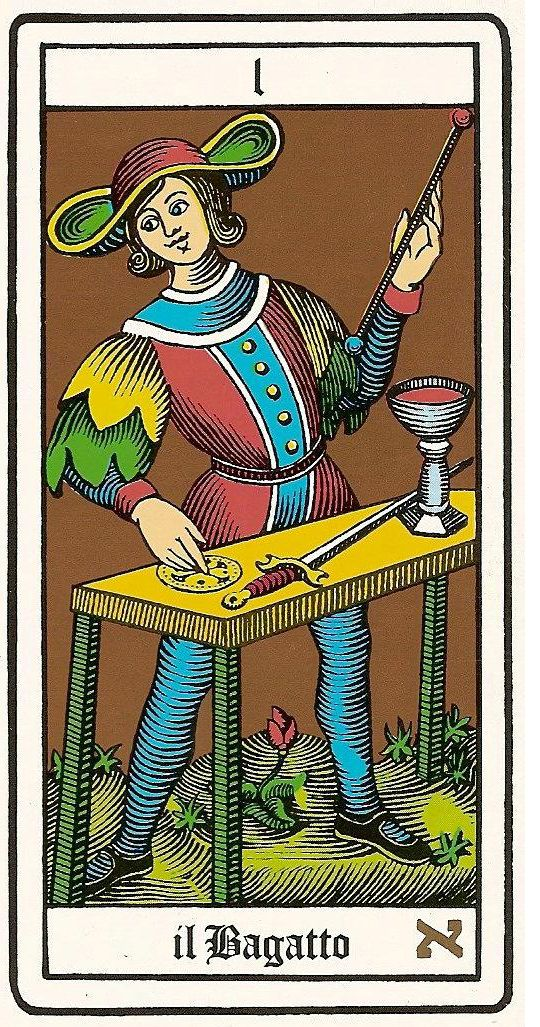
\includegraphics[width=.4\textwidth]{Il_bagatto.jpeg}

\caption{Bagatto, carta numero uno dei tarocchi}

\label{fig:il bagatto}

\end{center}

\end{figure}
